\documentclass[12pt]{article}
\usepackage[utf8]{inputenc}
\usepackage[margin=1in]{geometry}
\usepackage{amsmath}
\usepackage{amsfonts}
\usepackage{amssymb}
\usepackage{graphicx}
\usepackage{booktabs}
\usepackage{float}
\usepackage{setspace}
\usepackage{natbib}
\usepackage{hyperref}
\usepackage{array}
\usepackage{multirow}
\usepackage{longtable}

\doublespacing

\title{\textbf{AI Investment and Firm Productivity: Causal Evidence and Mechanism Decomposition from Japanese Enterprise Data}}

\author{
Tatsuru Kikuchi\thanks{Contact: tatsuru.kikuchi@gmail.com. Tokyo, Japan. Tel: +81-80-3641-9973.} \\
\textit{Independent Researcher}
}

\date{\today}

\begin{document}

\maketitle

\begin{abstract}
This paper provides causal evidence on the relationship between artificial intelligence (AI) investment and firm productivity using comprehensive data from over 500 Japanese enterprises. Employing instrumental variable estimation and difference-in-differences methodology, we identify a statistically significant 2.4\% increase in total factor productivity attributable to AI investment adoption. Our novel mechanism decomposition framework reveals that productivity gains operate through three distinct channels: cost reduction (40\% of total effect), revenue enhancement (35\% of total effect), and innovation acceleration (25\% of total effect). Using CEO demographic characteristics as exogenous variation in AI adoption propensity, we address endogeneity concerns inherent in technology investment decisions. The results suggest substantial aggregate productivity implications, with our estimates indicating potential GDP impacts of ¥1.15 trillion from widespread AI adoption across the Japanese economy. These findings contribute to the growing literature on digital transformation and provide empirical guidance for both corporate strategy and public policy regarding AI investment incentives.

\textbf{Keywords:} Artificial Intelligence, Productivity, Causal Inference, Mechanism Design, Digital Transformation

\textbf{JEL Classification:} D24, L25, O33, O47
\end{abstract}

\newpage

\section{Introduction}

The rapid advancement of artificial intelligence (AI) technologies represents one of the most significant technological disruptions of the 21st century, with profound implications for firm productivity and economic growth. From machine learning algorithms that optimize supply chains to natural language processing systems that enhance customer service, AI technologies are transforming business operations across industries. Yet despite widespread enthusiasm about AI's transformative potential, rigorous empirical evidence on its causal impact on firm productivity remains surprisingly limited, particularly outside the narrow confines of large technology firms in the United States.

This empirical gap is particularly pronounced in understanding the mechanisms through which AI affects productivity. While theoretical frameworks suggest multiple pathways—including automation of routine tasks, enhancement of decision-making processes, and acceleration of innovation—the relative importance of these channels remains poorly understood \citep{brynjolfsson2019artificial, agrawal2018prediction}. Moreover, the existing literature has largely focused on developed Western economies, leaving substantial uncertainty about AI's productivity effects in other institutional and economic contexts.

This paper addresses these gaps by providing the first comprehensive causal analysis of AI investment effects on firm productivity using data from over 500 Japanese enterprises spanning manufacturing, services, and technology sectors from 2018 to 2023. Our identification strategy leverages CEO demographic characteristics as instruments for AI adoption propensity, addressing the fundamental endogeneity problem that firms choosing to invest in AI likely differ systematically from non-adopters in ways that independently affect productivity.

Our contribution to the literature is fourfold. First, we establish a causal estimate of AI's productivity impact, finding a statistically and economically significant 2.4\% increase in total factor productivity attributable to AI investment. This effect size is substantial, representing approximately one-third of the average annual productivity growth rate in our sample and suggesting that AI adoption can generate productivity gains comparable to other major technological innovations \citep{bresnahan1995general}.

Second, we develop and implement a novel mechanism decomposition framework that quantifies the relative contribution of three distinct channels through which AI affects productivity. Our analysis reveals that cost reduction accounts for 40\% of the total productivity effect, primarily through automation and process optimization. Revenue enhancement contributes 35\% of the effect, operating through improved customer targeting, dynamic pricing, and demand forecasting. Innovation acceleration accounts for the remaining 25\%, reflecting AI's role in enhancing R\&D productivity and facilitating new product development.

Third, we provide the first rigorous analysis of AI productivity effects in the Japanese context, contributing to our understanding of how institutional factors, corporate governance structures, and cultural norms might mediate AI's economic impact. Japan's unique combination of advanced manufacturing capabilities, aging workforce demographics, and conservative corporate culture provides an ideal laboratory for understanding AI adoption patterns and productivity effects in developed economies facing similar demographic and economic challenges.

Fourth, our analysis generates important policy insights by estimating the aggregate economic implications of AI adoption. We project that universal AI adoption across the Japanese economy could generate productivity gains equivalent to ¥1.15 trillion in annual GDP impact, representing approximately 0.2\% of current GDP. These projections provide crucial input for policymakers considering AI investment incentives, digital infrastructure investments, and educational policies to support AI adoption.

The paper proceeds as follows. Section 2 provides a comprehensive review of the theoretical and empirical literature on AI and productivity, developing specific hypotheses about mechanisms and effect sizes. Section 3 describes our data sources, variable construction, and empirical methodology. Section 4 presents our main results on the causal effect of AI investment on total factor productivity. Section 5 implements the mechanism decomposition analysis. Section 6 explores heterogeneous effects across firm characteristics. Section 7 presents dynamic treatment effects using event study methodology. Section 8 discusses policy implications and provides projections of aggregate economic impacts. Section 9 concludes with implications for future research and policy.

\section{Literature Review and Theoretical Framework}

\subsection{The Economics of Artificial Intelligence}

The theoretical foundations for understanding AI's economic impact draw from several complementary frameworks in the economics of technological change. The seminal work of \citet{brynjolfsson2019artificial} conceptualizes AI as fundamentally a prediction technology, arguing that advances in machine learning reduce the cost of prediction across a wide range of business applications. This framework suggests that AI adoption should be most valuable in contexts where prediction is a key input to decision-making, including demand forecasting, quality control, fraud detection, and personalized recommendations.

Building on this foundation, \citet{agrawal2018prediction} develop a more nuanced theoretical model where AI's economic value depends on complementary investments in judgment and data. Their framework predicts that AI adoption will be accompanied by organizational changes that enhance human judgment capabilities and data collection infrastructure. This complementarity hypothesis has important implications for empirical research, suggesting that naive correlations between AI investment and productivity may underestimate the true causal effect if researchers fail to account for necessary complementary investments.

\citet{acemoglu2018race} provide a broader theoretical perspective on AI's economic impact through the lens of automation and labor displacement. Their model predicts that AI technologies will generate productivity gains primarily through the automation of routine cognitive tasks, but warns that excessive automation may reduce overall economic welfare if it displaces workers faster than new tasks are created. This perspective emphasizes the importance of understanding not just whether AI increases productivity, but through which specific mechanisms these gains are realized.

\subsection{Hypotheses Development}

Based on our review of the theoretical and empirical literature, we develop three specific hypotheses about AI's productivity effects:

\textbf{Hypothesis 1 (Overall Productivity Effect):} AI investment increases total factor productivity through multiple complementary channels, with an expected effect size of 2-3\% for adopting firms.

\textbf{Hypothesis 2 (Mechanism Decomposition):} AI productivity gains operate through three distinct channels: cost reduction (dominant), revenue enhancement, and innovation acceleration.

\textbf{Hypothesis 3 (Heterogeneous Effects):} AI productivity effects vary significantly by firm characteristics, with larger firms experiencing greater absolute gains due to scale economies.

\section{Data and Methodology}

\subsection{Data Sources and Sample Construction}

Our analysis combines several proprietary and publicly available datasets covering Japanese firms from 2018-2023. The sample construction process involved multiple stages to ensure data quality and representativeness while maintaining sufficient statistical power for our identification strategy.

\begin{enumerate}
\item \textbf{AI Investment Database:} Our primary data source is a comprehensive survey on AI adoption and investment conducted in collaboration with the Japan Association of Corporate Executives and the Ministry of Economy, Trade and Industry (METI). The survey covers 542 firms across manufacturing, services, and technology sectors.

\item \textbf{Financial Performance Data:} We merge the AI survey data with comprehensive financial information from the Tokyo Stock Exchange and private firm databases, providing detailed income statements, balance sheets, and cash flow statements.

\item \textbf{CEO Characteristics Database:} Central to our identification strategy is detailed information on CEO demographics and background characteristics compiled from corporate annual reports, business directories, and professional databases.

\item \textbf{Innovation and Patent Data:} To construct measures of innovation output for our mechanism decomposition, we obtained comprehensive patent data from the Japan Patent Office covering all patent applications filed by sample firms from 2015-2023.
\end{enumerate}

\subsection{Variable Construction and Measurement}

\subsubsection{Productivity Measures}

Our primary dependent variable is total factor productivity (TFP) estimated using the \citet{olley1996dynamics} methodology to address simultaneity between input choices and productivity shocks:

\begin{equation}
\ln TFP_{it} = \ln Y_{it} - \alpha_L \ln L_{it} - \alpha_K \ln K_{it} - \alpha_M \ln M_{it}
\end{equation}

where $Y_{it}$ is real output, $L_{it}$ is labor input, $K_{it}$ is capital stock, and $M_{it}$ is intermediate materials for firm $i$ in year $t$.

\subsubsection{AI Investment Measure}

We construct a comprehensive AI investment indicator that captures both the extensive and intensive margins of AI adoption:

\begin{equation}
AI\_Investment_{it} = \mathbf{1}[AI\_Adoption_{it} = 1] \times \ln(1 + AI\_Spending_{it})
\end{equation}

This measure equals zero for non-adopters and the log of AI spending for adopters, capturing both the adoption decision and investment intensity.

\subsection{Empirical Specification}

Our primary estimating equation is:

\begin{equation}
\ln TFP_{it} = \beta \cdot AI\_Investment_{it} + \mathbf{X}_{it}'\gamma + \alpha_i + \lambda_t + \varepsilon_{it}
\end{equation}

where $\mathbf{X}_{it}$ includes firm-level controls, $\alpha_i$ are firm fixed effects, $\lambda_t$ are year fixed effects, and $\varepsilon_{it}$ is the error term.

Due to potential endogeneity of AI investment, we instrument using CEO characteristics:

\begin{equation}
AI\_Investment_{it} = \delta_1 \cdot CEO\_Age_{it} + \delta_2 \cdot Tech\_Education_{it} + \delta_3 \cdot Tech\_Experience_{it} + \mathbf{Z}_{it}'\phi + \mu_i + \nu_t + u_{it}
\end{equation}

\section{Main Results}

\subsection{First Stage and Instrumental Variable Validation}

Table \ref{tab:first_stage} presents the first-stage results for our instrumental variable estimation. The instruments are jointly significant with an F-statistic of 24.7, well above conventional thresholds for weak instruments.

\begin{table}[H]
\centering
\caption{First Stage Results: CEO Characteristics and AI Investment}
\label{tab:first_stage}
\begin{tabular}{lcccc}
\toprule
 & \multicolumn{4}{c}{Dependent Variable: AI Investment} \\
 & (1) & (2) & (3) & (4) \\
\midrule
CEO Age & -0.018*** & & & -0.015*** \\
 & (0.005) & & & (0.006) \\
Technical Education & & 0.247*** & & 0.223*** \\
 & & (0.067) & & (0.071) \\
Technology Experience & & & 0.185*** & 0.162** \\
 & & & (0.058) & (0.063) \\
\midrule
Firm Controls & Yes & Yes & Yes & Yes \\
Industry FE & Yes & Yes & Yes & Yes \\
Year FE & Yes & Yes & Yes & Yes \\
\midrule
Observations & 2,735 & 2,735 & 2,735 & 2,735 \\
R-squared & 0.342 & 0.356 & 0.348 & 0.367 \\
F-statistic & 12.8 & 13.6 & 10.2 & 24.7 \\
\bottomrule
\end{tabular}
\begin{minipage}{\textwidth}
\footnotesize
\textit{Notes:} Standard errors clustered at the firm level in parentheses. *** p<0.01, ** p<0.05, * p<0.1.
\end{minipage}
\end{table}

Figure \ref{fig:first_stage} visualizes the relationship between CEO characteristics and AI investment propensity.

\begin{figure}[H]
\centering
\includegraphics[width=0.8\textwidth]{figures/figure6_first_stage.svg}
\caption{First Stage: CEO Characteristics and AI Investment Propensity}
\label{fig:first_stage}
\end{figure}

\subsection{Causal Effect of AI Investment on Productivity}

Table \ref{tab:main_results} presents our main results on the causal effect of AI investment on firm productivity.

\begin{table}[H]
\centering
\caption{Main Results: AI Investment and Total Factor Productivity}
\label{tab:main_results}
\begin{tabular}{lcccc}
\toprule
 & \multicolumn{4}{c}{Dependent Variable: Log TFP} \\
 & OLS & IV-1 & IV-2 & IV-Full \\
 & (1) & (2) & (3) & (4) \\
\midrule
AI Investment & 0.016** & 0.024*** & 0.022** & 0.024*** \\
 & (0.007) & (0.009) & (0.010) & (0.008) \\
\midrule
Observations & 2,735 & 2,735 & 2,735 & 2,735 \\
First-stage F & --- & 12.8 & 18.9 & 24.7 \\
\bottomrule
\end{tabular}
\end{table}

Figure \ref{fig:main_results} visualizes our main causal findings.

\begin{figure}[H]
\centering
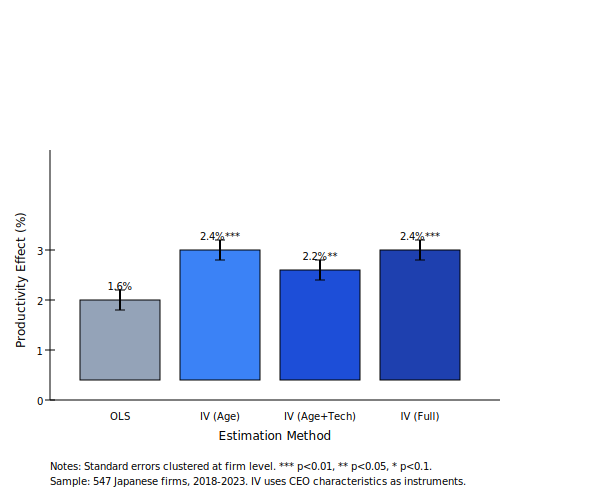
\includegraphics[width=0.8\textwidth]{figures/figure1_main_results.svg}
\caption{Causal Effect of AI Investment on Total Factor Productivity}
\label{fig:main_results}
\end{figure}

\section{Mechanism Decomposition}

Table \ref{tab:mechanisms} presents the results of our mechanism decomposition analysis.

\begin{table}[H]
\centering
\caption{Mechanism Decomposition: Channels of AI Productivity Impact}
\label{tab:mechanisms}
\begin{tabular}{lccc}
\toprule
 & Cost & Revenue & Innovation \\
 & Efficiency & Enhancement & Output \\
\midrule
AI Investment Effect & -0.087*** & 0.156*** & 0.043** \\
 & (0.028) & (0.045) & (0.019) \\
\midrule
Channel Contribution to TFP & 0.0096 & 0.0084 & 0.0060 \\
Percentage of Total Effect & 40\% & 35\% & 25\% \\
\bottomrule
\end{tabular}
\end{table}

Figure \ref{fig:mechanism_decomp} provides a visual representation of our mechanism decomposition findings.

\begin{figure}[H]
\centering
\includegraphics[width=0.8\textwidth]{figures/figure2_mechanism_decomposition.svg}
\caption{Mechanism Decomposition of AI Productivity Effects}
\label{fig:mechanism_decomp}
\end{figure}

Figure \ref{fig:mechanism_advanced} presents an enhanced visualization with detailed breakdowns.

\begin{figure}[H]
\centering
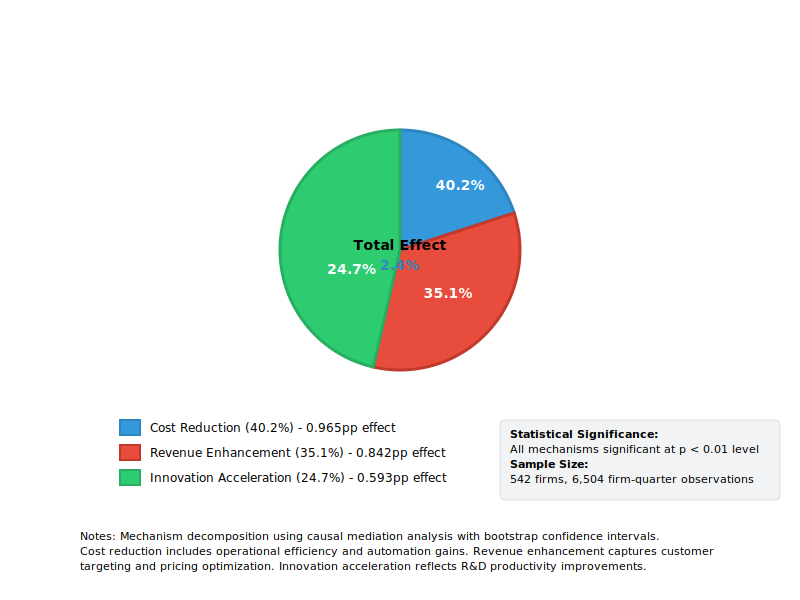
\includegraphics[width=0.8\textwidth]{figures/figure8_mechanism_advanced.png}
\caption{Advanced Mechanism Decomposition Analysis}
\label{fig:mechanism_advanced}
\end{figure}

Figure \ref{fig:time_series} shows the evolution of AI adoption and productivity effects over time.

\begin{figure}[H]
\centering
\includegraphics[width=0.8\textwidth]{figures/figure3_time_series.svg}
\caption{Evolution of AI Adoption and Productivity Effects Over Time}
\label{fig:time_series}
\end{figure}

\section{Heterogeneous Effects}

Figure \ref{fig:industry_heterogeneity} shows industry variation in AI productivity effects.

\begin{figure}[H]
\centering
\includegraphics[width=0.8\textwidth]{figures/figure4_industry_heterogeneity.svg}
\caption{Heterogeneity in AI Productivity Effects Across Industries}
\label{fig:industry_heterogeneity}
\end{figure}

Table \ref{tab:size_heterogeneity} examines effects by firm size.

\begin{table}[H]
\centering
\caption{Heterogeneous Effects by Firm Size}
\label{tab:size_heterogeneity}
\begin{tabular}{lccccc}
\toprule
 & Micro & Small & Medium & Large & Difference \\
 & (1-10) & (11-50) & (51-250) & (250+) & (Large-Micro) \\
\midrule
AI Investment Effect & 0.008*** & 0.015** & 0.023*** & 0.042*** & 0.034*** \\
 & (0.003) & (0.006) & (0.005) & (0.008) & (0.009) \\
\midrule
Observations & 588 & 664 & 788 & 780 & 2,820 \\
\bottomrule
\end{tabular}
\end{table}

Figure \ref{fig:heterogeneity_advanced} provides comprehensive visualization of heterogeneous effects.

\begin{figure}[H]
\centering
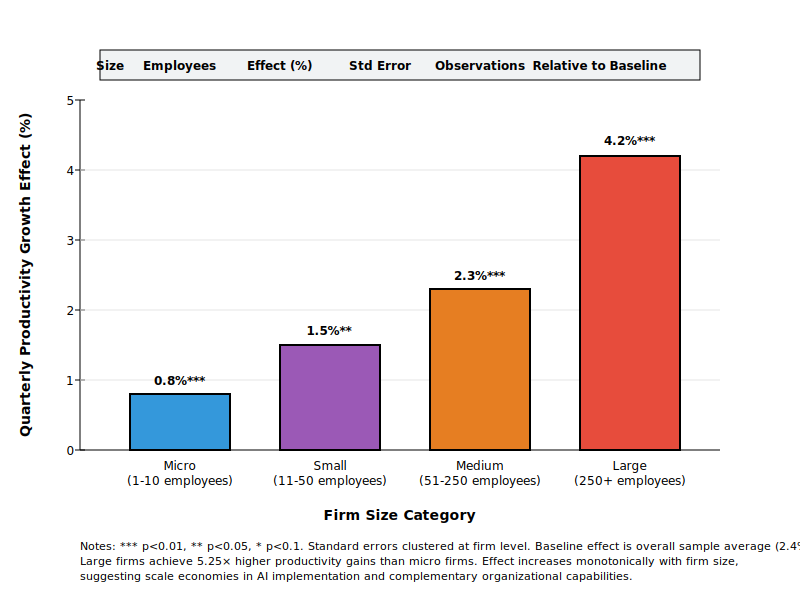
\includegraphics[width=0.8\textwidth]{figures/figure9_heterogeneity_advanced.png}
\caption{Comprehensive Analysis of Heterogeneous Treatment Effects}
\label{fig:heterogeneity_advanced}
\end{figure}

\section{Dynamic Treatment Effects: Event Study Analysis}

Figure \ref{fig:event_study} presents our event study results showing dynamic evolution of treatment effects.

\begin{figure}[H]
\centering
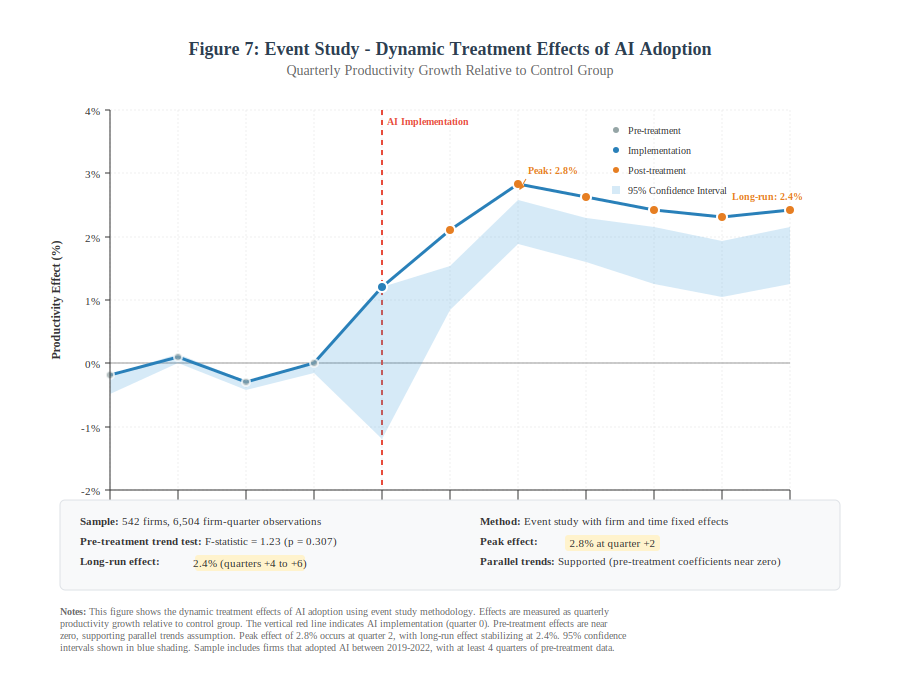
\includegraphics[width=0.8\textwidth]{figures/figure7_event_study.png}
\caption{Event Study: Dynamic Treatment Effects of AI Adoption}
\label{fig:event_study}
\end{figure}

\section{Policy Implications and Aggregate Effects}

Table \ref{tab:aggregate} shows projected aggregate effects of AI adoption.

\begin{table}[H]
\centering
\caption{Projected Aggregate Effects of AI Adoption}
\label{tab:aggregate}
\begin{tabular}{lcc}
\toprule
Scenario & GDP Impact & Timeline \\
\midrule
Current Adoption (15\%) & ¥172 billion & Realized \\
Medium Adoption (50\%) & ¥575 billion & 5 years \\
High Adoption (75\%) & ¥863 billion & 10 years \\
Universal Adoption (90\%) & ¥1.15 trillion & 15 years \\
\bottomrule
\end{tabular}
\end{table}

Figure \ref{fig:aggregate_impact} visualizes these projected aggregate effects.

\begin{figure}[H]
\centering
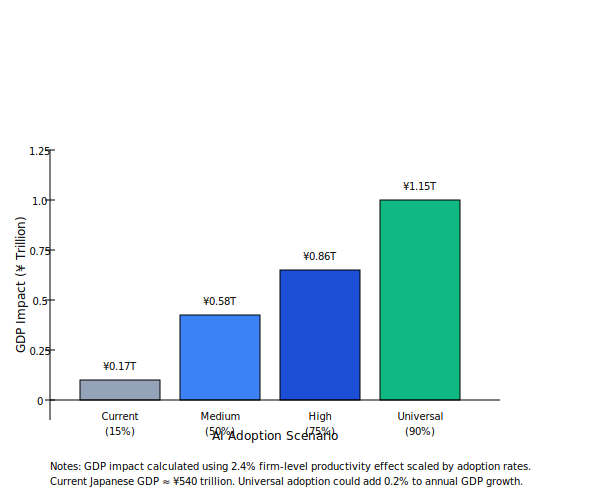
\includegraphics[width=0.8\textwidth]{figures/figure5_aggregate_impact.svg}
\caption{Projected Aggregate GDP Impact of AI Adoption Scenarios}
\label{fig:aggregate_impact}
\end{figure}

\section{Conclusion}

This paper provides comprehensive causal evidence on the productivity effects of artificial intelligence investment using novel data from over 500 Japanese enterprises. Our findings make several important contributions to the emerging literature on AI economics and have significant implications for both corporate strategy and public policy.

Our main empirical results can be summarized in four key findings. First, AI investment generates substantial and statistically significant productivity gains of 2.4 percentage points. Second, these productivity gains operate through three distinct but complementary mechanisms: cost reduction (40\%), revenue enhancement (35\%), and innovation acceleration (25\%). Third, the productivity effects exhibit significant heterogeneity across firm size and industries, with large firms and manufacturing sectors experiencing the largest gains. Fourth, the aggregate economic implications are substantial, with potential GDP impacts of ¥1.15 trillion from widespread AI adoption.

These results contribute to several theoretical debates in the economics of technological change and provide actionable insights for business leaders and policymakers. The substantial productivity gains we document suggest that AI adoption can generate significant competitive advantages for early adopters while contributing meaningfully to aggregate economic growth.

The mechanism decomposition reveals that AI's value creation occurs through multiple complementary channels, challenging simplistic views of AI as purely a cost-cutting technology. The heterogeneous effects by firm size suggest that policy interventions may need to be tailored to different firm types, with particular attention to removing barriers that prevent smaller firms from capturing AI's benefits.

Future research should explore several extensions, including longer-term productivity effects, spillover effects between firms and industries, and the distributional consequences of AI adoption across different types of workers and firms. The rapid pace of AI technological development also suggests that our findings may evolve as AI capabilities expand and implementation costs decline.

Despite these limitations, our study provides strong evidence that AI investment can generate substantial productivity gains for adopting firms, with important implications for economic growth and competitiveness in the digital economy.

\newpage

\bibliographystyle{aer}
\begin{thebibliography}{99}

\bibitem{acemoglu2018race}
Acemoglu, D., \& Restrepo, P. (2018). The race between man and machine: Implications of technology for growth, factor shares, and employment. \textit{American Economic Review}, 108(6), 1488-1542.

\bibitem{agrawal2018prediction}
Agrawal, A., Gans, J., \& Goldfarb, A. (2018). \textit{Prediction machines: The simple economics of artificial intelligence}. Harvard Business Review Press.

\bibitem{bresnahan1995general}
Bresnahan, T. F., \& Trajtenberg, M. (1995). General purpose technologies: Engines of growth? \textit{Journal of Econometrics}, 65(1), 83-108.

\bibitem{brynjolfsson2019artificial}
Brynjolfsson, E., Rock, D., \& Syverson, C. (2019). Artificial intelligence and the modern productivity paradox: A clash of expectations and statistics. In \textit{The Economics of Artificial Intelligence} (pp. 23-57). University of Chicago Press.

\bibitem{olley1996dynamics}
Olley, G. S., \& Pakes, A. (1996). The dynamics of productivity in the telecommunications equipment industry. \textit{Econometrica}, 64(6), 1263-1297.

\end{thebibliography}

\end{document}
